% -*- root: ../assignment.tex -*-

\subsection*{Singular Value Decomposition}
\begin{enumerate}[resume]
    \item For a square $\mf{A} \in\mb{R}^{n \times n}$, the SVD tells us how a unit sphere in $\mb{R}^n$ is distorted by the linear transformation performed by $\mf{A}$. This degree of distortion can be quantified using the singular values of $\mf{A}$, which is the 2-norm \textit{condition number},
    \[ \kappa = \frac{\sigma_1}{\sigma_n} \]
    \begin{enumerate}
        \item Explain why $\kappa \geq 1$?
        \item What is condition number of a singular matrix?
        \item If $\mf{A}$ is non-singular, show that $\kappa = \lV\mf{A}\rV_2\lV\mf{A}^{-1}\rV_2$
        \item Condition numbers can also be defined based on other p-norms. The general p-norm condition number is given by, $\kappa_p = \lV\mf{A}\rV_p\lV\mf{A}^{-1}\rV_p$. Evaluate the 1-norm, 2-norm and $\infty$-norm condition numbers for the following matrices. How do these number compare with each other?
        \begin{enumerate*}[label={(\roman*)}]
            \item $\mf{A} = \bmx 1 & 0\\ 0 & 1\emx$;
            \item $\mf{A} = \bmx 1 & -1\\ 10 & -9\emx$;
            \item $\mf{A} = \bmx 1 & 5\\ -1 & 1\emx$.
        \end{enumerate*}
        \item Conditions numbers play an important role in practice. We had earlier an example of an ill-conditioned system $\mf{Ax} = \mf{b}$ (problem \ref{matrices:uncertain}). Consider the following systems, where:
        \begin{enumerate*}[label={(\roman*)}]
            \item $\mf{A}_1 = \bmx 1 & -1 \\ 10 & -9\emx$; and 
            \item $\mf{A}_2 = \bmx 1 & -10 \\ 1 & 10\emx$
         \end{enumerate*}.

        For $\mf{b} = \bmx 10 \\ 0\emx$, what are the solutions $\mf{x}_1\lp=\mf{A}_1^{-1}\mf{b}\rp$ and $\mf{x}_2\lp=\mf{A}_2^{-1}\mf{b}\rp$? 

        Suppose there is an error in the measurement of $\mf{b}$, and we have $\tilde{\mf{b}} = \bmx 9 \\ 1\emx$. The relative error in $\mf{b}$ is given by $\delta b = \frac{\lV \mf{b} - \tilde{\mf{b}}\rV_2}{\lV\mf{b}\rV_2}$. What are the new solutions $\tilde{\mf{x}}_1$ and $\tilde{\mf{x}}_2$?

        Calculate $\delta x_1$ and $\delta x_2$, the relative errors in $\mf{x}_1$ and $\mf{x}_2$, respectively? How do these compare to $\delta b$?

        \textit{Note: Through this problem, you should be able to see that an ill-conditioned system has a large condition number, which can amplify error and thus lead to large uncertainty in the solutions.}
    \end{enumerate}

    \item Consider a system  $S$, which when probed with a test signal $x\lp  t\rp$, and the system responds with an output signal $y\lp t\rp$. The experiment is repeated $M$ times on the system by repeatedly applying the text signal to th system and the response of the system is sampled $y\ls n\rs$ and recorded for a for a fixed duration of time $0 \leq n \leq N$. An example of the response of the system for the different experiments are shown below ($N = 100$),\vspace{-0.25cm}
    \begin{center}
    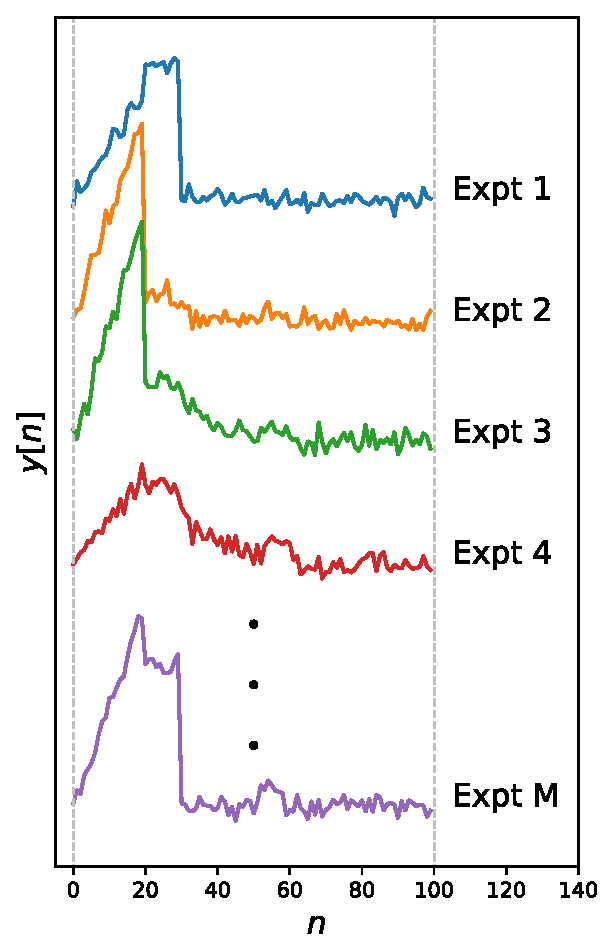
\includegraphics[width=0.7\columnwidth]{sections/figs/trig_expt.eps}
    \end{center}\vspace{-0.3cm}
    We know from the physics of the system that the system response to the test signal for the $j^{th}$ experiment given is given by ,
    \[ y_j\ls n \rs = \sum_{i=1}^{K} w_{ji}\phi_i\ls n\rs + \nu_j\ls n\rs\]
    where, $n$ is time index; $N$ is the number of data points recorded on each experiment; $\phi_i\ls n\rs, 1 \leq i \leq K$ are characteristic signals of the system; $w_{ji}$ are the weights that determine the amount of the $\phi_i$ present in the output $y_j$ for the $j^{th}$ experiment; and $\nu_j\ls n\rs$ is measurement noise present in the $j^{th}$ experiments. Additionally, we also know that
    $$ \phi_i^T\phi_j = \sum_{l=0}^{N-1} \phi_i\ls l \rs\phi_j\ls l\rs = \begin{cases} 0 & i \neq j \\ 1 & i = j \end{cases} $$

    Data from one such experiment is provided in the CSV file (trigexpt.csv) which contains an array of data where the rows correspond to system response for the different experiments, and the columns correspond to  different time index. Using this data identify the different characteristic signals $\phi_i$ for the system, along with the weights $w_{ji}$ for the different experiments. You must also ensure that the data is explained with least number characteristic signal, i.e. $K$ should be as low as possible. Explain how you chose $K$.l
\end{enumerate}
% \vfill